%% VEIN manuscript --- Springer Nature article class (sn-jnl).
%% Author-year reference style (sn-mathphys-ay); referee option = double spacing.
\documentclass[referee,pdflatex,sn-mathphys-ay]{sn-jnl}

\usepackage{graphicx}%
\usepackage{multirow}%
\usepackage{amsmath,amssymb,amsfonts}%
\usepackage{amsthm}%
\usepackage{mathrsfs}%
\usepackage[title]{appendix}%
\usepackage{xcolor}%
\usepackage{textcomp}%
\usepackage{manyfoot}%
\usepackage{booktabs}%
\usepackage{algorithm}%
\usepackage{algorithmicx}%
\usepackage{algpseudocode}%
\usepackage{enumitem}%

\theoremstyle{thmstyleone}%
\newtheorem{theorem}{Theorem}%
\newtheorem{proposition}[theorem]{Proposition}%
\theoremstyle{thmstyletwo}%
\newtheorem{example}{Example}%
\newtheorem{remark}{Remark}%
\theoremstyle{thmstylethree}%
\newtheorem{definition}{Definition}%
\newtheorem{assumption}{Assumption}%

\newcommand{\doop}{\mathrm{do}}
\newcommand{\pa}{\mathrm{pa}}
\newcommand{\VaR}{\mathrm{VaR}}
\newcommand{\E}{\mathbb{E}}
\newcommand{\OCCoVaR}{\text{OC-CoVaR}}

\graphicspath{{figures/}}
\raggedbottom

\begin{document}

\title[VEIN: On-Chain Causal Risk Attribution]{VEIN: On-Chain Causal Risk
Attribution for Cryptocurrency Systemic Risk}

\author*[1]{\fnm{Author} \sur{information withheld for peer review}}
\affil*[1]{\orgname{Affiliation withheld for peer review}}

\abstract{Return-based causal measures of cryptocurrency systemic risk infer
the contagion graph \emph{statistically}, from price co-movement, using
constraint-based structure learning or directed-information estimation; the
mechanism of transmission---which entity actually moved funds into
distress---stays unobserved. We propose VEIN (Verifiable Entity-resolved
Interventional/counterfactual Network risk), a framework that instead treats
the resolved on-chain transaction ledger as an \emph{auditable candidate
structural skeleton}: under explicit edge-type and timing assumptions, the
in-neighbours of an entity in this entity-resolved graph specify the parent
set of a Pearl-style structural causal model (SCM), rather than a parent set
inferred from correlations. On this skeleton VEIN defines an interventional
risk measure (On-Chain Causal CoVaR) through the do-operator and, to our
knowledge, the first on-chain counterfactual (Pearl Level-3) systemic-risk
\emph{attribution} measure proposed for crypto markets, which decomposes a
realised loss into the Shapley-exact share attributable to each upstream
entity's distress. We implement the complete pipeline---a four-tier
entity-resolution layer over Dune Analytics' decoded Ethereum tables, the SCM,
and the risk measures---and evaluate it on real on-chain data around the
October~2025 cascading liquidation event, one of the largest documented
deleveraging episodes in crypto markets, with generality checks on the FTX
(2022) and USDC/SVB (2023) stress episodes. The primary contribution is this
attribution measure: it yields an exact, order-robust decomposition of
realised losses into upstream entities, and produces systemic-importance
rankings that diverge from $\Delta$CoVaR and MES (Spearman $\rho=0.52$),
survive removing the retail aggregate, and are stable under coefficient
perturbation (Spearman $0.88$). One-step prediction is a secondary,
graph-source ablation under common VEIN equations, not a replication of
TV-DIG or Causal-NECO VaR: at the cascade's hourly timescale the observed
graph is competitive with a price-estimated Granger graph (better in $71\%$
of paired bootstrap resamples) but the edge is not decisive---it does not
survive a strict lagged-flow forecast or a price-based stress target---so we
report this comparison as suggestive rather than established. The directional
content of flow edges is event- and edge-type-conditional: reversal degrades
one-step prediction in the FTX and USDC/SVB episodes and, on a leakage-free
non-flow stress target built from prices and pegs alone, by $\approx9\%$,
confirming the signal is not an artefact of flow-defined stress; it washes
out into near-symmetry only in the custodial-settlement-dominated
October-2025 cascade, where connectivity rather than direction appears to
carry the systemic content. A validity and falsification battery
(placebo/negative controls, unobserved-confounding robustness values,
resolution robustness, and external validity against the documented
narrative) supports these components while delimiting the off-chain-CEX and
entity-resolution limits that any ledger-only analysis inherits. We discuss
the implications for regulators and the limits imposed by centralised-exchange
opacity. JEL classification: G01, G17, G18, C58.}

\keywords{systemic risk, cryptocurrency, structural causal models,
counterfactual inference, blockchain, CoVaR, contagion}

\maketitle

\section{Introduction}
\label{sec:intro}

On 10--11 October 2025, cryptocurrency markets experienced the largest
deleveraging event in their history: on the order of nineteen billion US
dollars of leveraged positions were liquidated within thirty-six
hours.\footnote{For event overviews and the minute-level liquidation mechanics,
see CoinDesk Research, \url{https://www.coindesk.com/research/market-spotlight-the-19-billion-liquidation-that-shook-crypto};
CoinGecko, \url{https://www.coingecko.com/learn/october-10-crypto-crash-explained};
and FTI Consulting, \url{https://www.fticonsulting.com/insights/articles/crypto-crash-october-2025-leverage-met-liquidity}.}
Early scholarly post-mortems of the episode \citep{ali2025anatomy,lim2026cascade}
document a striking feature that sets it apart from the 2022 episodes
(Terra/Luna, Celsius, FTX): whereas those were rooted in fundamental
insolvency, the October~2025 cascade was largely \emph{mechanical}. A mispricing
in a centralised exchange's internal valuation engine\footnote{The proximate
trigger has been attributed to Binance's unified-account margin system, which
valued posted collateral (including USDe, wBETH and BNSOL) using its own
internal spot prices rather than external oracles; see
\url{https://www.ccn.com/education/crypto/ethena-usde-depeg-binance-crash-explained/}
and \url{https://ambcrypto.com/not-a-true-depeg-says-ethena-founder-as-usde-faces-binance-only-slip/}.}
propagated into automated liquidations, which in turn forced sales that
depressed prices and triggered further liquidations---a classic
funding-liquidity spiral operating at machine speed. A defining feature was
architectural: decentralised finance (DeFi) lending protocols with transparent,
over-collateralised positions (e.g.\ Aave) emerged with essentially zero bad
debt, whereas centralised-exchange (CEX) risk engines amplified the shock. The
synchronised depeg of the synthetic dollar USDe---which remained fully solvent
throughout, so that the depeg was a pricing and liquidity artefact rather than a
default---is emblematic of this architecture-dependent
fragility.\footnote{USDe's price fell to roughly \$0.65 on Binance while holding
near \$1 on other venues and in DeFi, and remained redeemable as supply
contracted from about \$9bn to \$6bn, confirming an exchange-specific pricing
artefact rather than insolvency; see CoinDesk,
\url{https://www.coindesk.com/markets/2025/10/11/ethena-s-usde-briefly-loses-peg-during-usd19b-crypto-liquidation-cascade}
and \url{https://www.coindesk.com/markets/2025/10/13/no-ethena-s-usde-didn-t-de-peg}.}
Crucially for risk measurement, the proximate mechanism left a high-resolution
footprint \emph{on chain}: liquidation transfers, collateral movements, and
exchange in/out-flows are all recorded, timestamped to the block, in a public
ledger.

Such episodes expose a structural weakness in how systemic risk is measured for
crypto markets. The dominant tools---the change in Value-at-Risk conditional on
distress ($\Delta$CoVaR, for Conditional Value-at-Risk) \citep{adrian2016covar},
marginal expected shortfall (MES) and SRISK \citep{acharya2017measuring}, and
variance-decomposition connectedness
\citep{diebold2014network,billio2012econometric}---are \emph{associational}:
they quantify co-movement in returns and, as their own authors note, capture an
institution's contribution to system risk ``in a non-causal sense''
\citep{adrian2016covar}. A recent and comprehensive survey of causal inference in
finance \citep{kumar2025causalreview} confirms the pattern at the level of the
whole field: applications around SRISK, MES and CoVaR remain confined to
association and Granger causality, with no counterfactual systemic-risk measure.
Where causality has been injected, the graph is still \emph{estimated from
prices}. Causal-NECO VaR \citep{rigana2024neco,rigana2023new} learns a contagion
graph from foreign-exchange returns using the order-independent PC-stable
algorithm (a constraint-based causal-structure-discovery algorithm)
\citep{colombo2014order,spirtes2000causation} and computes a
value-at-risk from the resulting SCM; the time-varying directed-information
graph (TV-DIG) of Etesami et al.\ \citeyearpar{etesami2023tvdig} builds directed
networks---an information-theoretic generalisation of Granger causality
\citep{granger1969}---across financial sectors including cryptocurrencies; and
correlation-network models such as CoRisk \citep{giudici2018corisk} decompose
systemic risk into idiosyncratic and contagion components. The crypto-specific
literature has grown rapidly in 2025--2026, from composite indices such as ASRI
\citep{farzulla2026asri} to network-fragility and TradFi--DeFi
``crosstagion'' mappings \citep{aufiero2025mapping}; yet all of this work either
estimates the network from returns or treats the on-chain graph descriptively.
No published method exploits the one data source where the contagion mechanism
is \emph{directly observed}---the blockchain ledger---as a causal structure.

On-chain transaction graphs have, separately, been used for prediction and
forensics---``chainlets'' that forecast Bitcoin price and volatility
\citep{akcora2018bitcoin}, and address-clustering for anti-money-laundering
\citep{meiklejohn2013fistful,weber2019antimoney}---but always observationally,
explicitly disclaiming a causal-structural interpretation, and never as the
backbone of a systemic-risk measure. And although Pearl's causal hierarchy
\citep{pearl2009causality,pearl2019seven} places counterfactuals (Level~3) above
interventions (Level~2) above association (Level~1), no systemic-risk measure in
finance operates above Level~2. There is, in short, an open intersection: an
observed-graph SCM for crypto systemic risk, extended to the counterfactual
level. This paper occupies it.

We make three contributions. First, we propose VEIN, which treats the
entity-resolved on-chain transaction graph as an \emph{auditable candidate
structural skeleton} for a Pearl SCM: under explicit edge-type and timing
assumptions (A1--A3, Section~\ref{sec:method}), the in-neighbour set $\pa(i)$
of each entity is \emph{specified from the resolved ledger} rather than
inferred from price correlations; block timestamps make the temporal ordering
of on-chain transactions observable, reducing---though not eliminating---the
timing ambiguity that price-based methods must instead assume away. Second, we define
On-Chain Causal CoVaR (OC-CoVaR), an interventional (Level-2) measure via the
do-operator, together with a counterfactual (Level-3) attribution measure that
decomposes a
realised loss into the share attributable to a specific upstream entity through
the standard abduction--action--prediction procedure. Third, we implement the
full pipeline---including a four-tier entity-resolution layer over real decoded
Ethereum data---and evaluate it on the October~2025 event against
price-estimated graphs and standard non-causal baselines, subjecting every
causal claim to a falsification and validity battery and reporting negative
results as readily as positive ones. The evaluation is organised around the five
hypotheses in Table~\ref{tab:hyp}, each paired in Section~\ref{sec:results} with
the test and falsification criterion that would overturn it.

\begin{table}[t]
\centering
\small
\caption{Hypotheses evaluated in this paper.}
\label{tab:hyp}
\begin{tabular}{@{}p{0.06\linewidth}p{0.84\linewidth}@{}}
\toprule
\textbf{ID} & \textbf{Statement}\\
\midrule
H1 & The observed on-chain flow graph predicts stress propagation more accurately than a graph statistically estimated from price returns.\\
H2a & In custodial settlement networks, connectivity rather than flow direction predicts stress propagation (edge reversal is near-neutral).\\
H2b & In directional, failure-origin or depeg events, reversing flow-edge direction degrades predictive accuracy (assumption A3 holds).\\
H3 & OC-CoVaR identifies a different set of systemically important entities than $\Delta$CoVaR/MES applied to returns.\\
H4 & The counterfactual measure decomposes the October~2025 losses into mechanically interpretable components.\\
H5 & On-chain composability/collateral edges add loss-attribution information beyond price correlation.\\
\bottomrule
\end{tabular}
\end{table}

The remainder of the paper is organised as follows.
Section~\ref{sec:related} positions VEIN against the causal and on-chain
literatures. Section~\ref{sec:method} develops the framework formally.
Section~\ref{sec:data} describes the data and the entity-resolution pipeline.
Section~\ref{sec:results} reports the empirical evaluation and validity battery.
Section~\ref{sec:discussion} discusses implications, limitations, and
conclusions. An appendix collects implementation details and additional tables.

\section{Related Work and Positioning}
\label{sec:related}

The systemic-risk literature begins with associational, return-based measures.
The canonical conditional measure is $\Delta$CoVaR \citep{adrian2016covar}, the
change in the value-at-risk of the financial system conditional on an
institution being in distress relative to its median state; the
systemic-expected-shortfall family \citep{acharya2017measuring} adds marginal
expected shortfall (MES) and the leverage-adjusted SRISK; and connectedness
measures built from forecast-error-variance decompositions
\citep{diebold2014network} or Granger-causal and correlation networks
\citep{billio2012econometric} quantify spillovers. These are, by construction,
descriptions of co-movement rather than of mechanism, and a recent survey of the
whole field \citep{kumar2025causalreview} confirms that even where the word
``causal'' appears, applications around CoVaR, MES and SRISK remain
associational or Granger-based.

The closest methodological precedent that genuinely estimates causal structure
is Causal-NECO VaR \citep{rigana2024neco}, which decomposes asset log-returns
into an autoregressive part and an instantaneous contagion part, learns the
causal graph with PC-stable \citep{colombo2014order}, and computes a Gaussian or
Gaussian-copula VaR. It operates at Pearl Levels~1--2 on foreign-exchange data,
assumes no unmeasured confounders, and---decisively for our purposes---obtains
its graph by estimation rather than observation; its foundational lineage
\citep{rigana2023new} combines causal networks with a structural vector
autoregression in Pearl's framework \citep{spirtes2000causation}. The nearest
crypto application is the time-varying directed-information graph TV-DIG
\citep{etesami2023tvdig}, a nonparametric directed network that detects
heightened crypto-to-sector influence around the 2022 stress events; directed
information generalises Granger causality \citep{granger1969} but is not a Pearl
SCM with do-operator and counterfactual semantics, and it too is built from
returns. The 2025--2026 crypto-specific wave---composite indices such as ASRI
\citep{farzulla2026asri} and comparative TradFi--DeFi systemic-risk mappings that
formalise composability-driven ``crosstagion'' \citep{aufiero2025mapping}---
sharpens the motivation but does not change the picture: the network is either
estimated from prices or treated descriptively.

On-chain transaction graphs themselves have been mined predictively, through
chainlet subgraphs that forecast Bitcoin price and volatility
\citep{akcora2018bitcoin}, and for forensics and address clustering, from the
multi-input/co-spend heuristics of \cite{meiklejohn2013fistful} to
graph-convolutional anti-money-laundering classifiers on the Elliptic dataset
\citep{weber2019antimoney}. We reuse this resolution machinery, but no prior work
treats the resulting graph as a causal structure for a systemic-risk measure.

Taken together, the literature leaves two specific capabilities unfilled, and a
deliberate survey of the most recent 2025--2026 work---the period in which one
might most expect the gap to have closed---confirms that it remains open. We
organise the evidence around the two sub-claims.

\emph{On the on-chain-graph-as-SCM claim.} The 2026 crypto systemic-risk
literature uses the on-chain graph descriptively or builds the network from
prices, never as a Pearl SCM. Sankaewtong \citeyearpar{sankaewtong2026tracing} traces
the USDC depeg contagion through high-granularity on-chain transactions, but
observationally, with no interventional or counterfactual semantics; Zhang et
al.\ \citeyearpar{zhang2026defi} measure DeFi systemic fragility from the
\emph{correlation} structure of total-value-locked dynamics; ASRI
\citep{farzulla2026asri} is an associational composite of weighted sub-indices;
and the comparative TradFi--DeFi ``crosstagion'' mapping of Aufiero et al.\
\citeyearpar{aufiero2025mapping} is conceptual. The detailed forensic reconstructions
of the very event we study---Lim's minute-level analysis \citeyearpar{lim2026cascade}
and Ali's anatomy \citeyearpar{ali2025anatomy}---characterise the mechanism but build
no causal risk measure. None reads the causal parent set off the ledger.

\emph{On the counterfactual-systemic-risk claim.} Counterfactual reasoning has
reached finance, but not systemic-risk measurement. Xu \citeyearpar{xu2025counterfactual}
applies counterfactual analysis to credit-portfolio losses, not to a networked
tail-risk measure; and the comprehensive 2025 survey of causal inference across
banking, finance and insurance by Kumar et al.\ \citeyearpar{kumar2025causalreview},
covering decades of work, documents only association and Granger usage around
SRISK, MES and CoVaR, with no counterfactual systemic-risk measure. The nearest
causal precedents---Causal-NECO VaR \citep{rigana2024neco} and TV-DIG
\citep{etesami2023tvdig}---stop at Pearl Level~2.

Against this 2026 state of the art, \emph{to the best of our knowledge VEIN is
the first framework to (i) use an observed on-chain transaction graph as a Pearl
structural causal model for a systemic-risk measure, and (ii) define a
counterfactual (Pearl Level-3) systemic-risk attribution measure in finance}.
Both sub-claims were checked against standard term combinations across arXiv,
SSRN and Semantic Scholar as of mid-2026 and returned no prior instance; as with
any negative existence claim they are bounded by search coverage, and we state
them as ``no evidence of'' rather than proof of absence. Table~\ref{tab:position}
situates VEIN against the nearest neighbours; throughout, we treat Causal-NECO
VaR (nearest method) and TV-DIG (nearest crypto application) as the reference
points, and we re-implement the estimated-graph approach on our own data as the
head-to-head baseline for H1.

\begin{table}[t]
\centering
\small
\caption{Positioning of VEIN against the nearest prior art.}
\label{tab:position}
\begin{tabular}{@{}p{0.26\linewidth}cccc@{}}
\toprule
\textbf{Method} & \textbf{Graph source} & \textbf{Causal level} & \textbf{Domain} & \textbf{Counterfactual}\\
\midrule
$\Delta$CoVaR \citep{adrian2016covar}     & none (returns)     & assoc.\ (L1) & general & no\\
MES/SRISK \citep{acharya2017measuring}    & none (returns)     & assoc.\ (L1) & general & no\\
CoRisk \citep{giudici2018corisk}          & corr.\ network     & assoc.\ (L1) & credit  & no\\
ASRI \citep{farzulla2026asri}             & composite index    & assoc.\ (L1) & crypto  & no\\
TV-DIG \citep{etesami2023tvdig}           & estimated (DI)     & Granger     & incl.\ crypto & no\\
Causal-NECO VaR \citep{rigana2024neco}    & estimated (PC)     & SCM (L1--2) & FX      & no\\
\textbf{VEIN (this paper)}               & \textbf{observed} & \textbf{SCM (L1--3)} & \textbf{crypto} & \textbf{yes}\\
\bottomrule
\end{tabular}
\end{table}

\section{The VEIN Framework}
\label{sec:method}

\subsection{Structural causal model and identification}
\label{subsec:scm}
Let $G=(V,E)$ be a directed, timestamped, dollar-weighted graph whose nodes $V$
are \emph{resolved economic entities} (exchanges, lending protocols, stablecoin
issuers, custodians, and an aggregate retail node) and whose edges $E$ are
observed on-chain flows. For each entity $i$ and discrete time $t$ we track a
scalar \emph{stress state} $S_{i,t}\in\mathbb{R}$, oriented so that larger means
more distressed; the realised flow $F_{p\to i,t}\ge0$ from $p$ to $i$ during
period $t$; and an exogenous shock $U_{i,t}$. Table~\ref{tab:notation}
summarises the notation. The defining structural equation of VEIN is
\begin{equation}
\label{eq:scm}
S_{i,t} \;=\; f_i\!\Big(S_{\pa(i),\,t-1},\; F_{\pa(i)\to i,\,t},\; U_{i,t}\Big),
\qquad
\pa(i) \;=\; \{\,p\in V : (p\to i)\in E\,\},
\end{equation}
The resolved ledger supplies an observed candidate propagation skeleton: under
the edge-type and timing assumptions A1--A3 below, the in-neighbours of $i$ in
$G$ are used to \emph{specify} the model parent set $\pa(i)$ of the SCM. This
is the central structural move of the paper: in contrast to
\citep{rigana2024neco,etesami2023tvdig}, $\pa(i)$ is specified from the ledger
rather than estimated from price correlations, so the only component requiring
statistical estimation is the stress-propagation function $f_i$; $\pa(i)$
carries a causal interpretation only insofar as A1--A3 hold for the edge types
and events under study, a claim we subject to direct falsification in
Section~\ref{subsec:h2valid}. We adopt a ridge-regularised linear
specification,
\begin{equation}
\label{eq:fi}
S_{i,t} \;=\; b_i + \sum_{p\in\pa(i)} a_{ip}\,S_{p,t-1}
            + \sum_{p\in\pa(i)} c_{ip}\,\log\!\big(1+F_{p\to i,t}\big)
            + U_{i,t},
\end{equation}
with parameters $\theta_i=(b_i,\{a_{ip}\},\{c_{ip}\})$ estimated by ridge
regression, $\hat\theta_i = \arg\min_{\theta_i} \sum_t (S_{i,t}-f_i(\cdot;\theta_i))^2
+ \lambda(\|a_{i\cdot}\|_2^2+\|c_{i\cdot}\|_2^2)$, on a pre-crisis estimation
window. The fitted residuals $\widehat U_{i,t}=S_{i,t}-f_i(\cdot;\hat\theta_i)$
furnish an empirical distribution of exogenous shocks used by the risk measures.

\begin{table}[t]
\centering
\small
\caption{Notation.}
\label{tab:notation}
\begin{tabular}{@{}ll@{}}
\toprule
\textbf{Symbol} & \textbf{Meaning}\\
\midrule
$G=(V,E)$ & resolved entity graph (nodes, directed flow edges)\\
$\pa(i)$ & model parent set of $i$, specified from in-neighbours in $G$\\
$S_{i,t}$ & stress state of entity $i$ at time $t$ ($z$-scored)\\
$F_{p\to i,t}$ & observed USD flow from $p$ to $i$ in period $t$\\
$U_{i,t}$ & exogenous shock to $i$ at $t$\\
$f_i$ & structural (stress-propagation) function of $i$\\
$L_j$ & loss functional of $j$ over the event window\\
$s^\ast$ & severe-distress intervention level ($95$th pctile)\\
$\Delta_i^{CF}(j)$ & counterfactual loss of $j$ attributable to $i$\\
$RV$ & confounding robustness value\\
\bottomrule
\end{tabular}
\end{table}

Because every parent enters \eqref{eq:fi} at lag $t\!-\!1$ in the stress term,
while the contemporaneous term depends only on the exogenous observed flows, the
multi-entity system is well posed even when $G$ contains directed cycles, as the
following observation makes precise.

\begin{proposition}[Well-posedness of the lagged system]
\label{prop:wellposed}
Given an initial state $S_{\cdot,0}$ and a shock path $\{U_{\cdot,t}\}$, the
trajectory $\{S_{\cdot,t}\}_{t\ge1}$ generated by \eqref{eq:fi} is uniquely
determined by forward iteration, even when $G$ contains directed cycles.
\end{proposition}
\begin{proof}[Proof sketch]
At step $t$ the right-hand side of \eqref{eq:fi} for every $i$ references only
quantities indexed at $t\!-\!1$ (parent stress) or exogenous quantities at $t$
(flows, shocks). There is therefore no simultaneity among the time-$t$ stress
variables, and $S_{\cdot,t}$ is computed in one vectorised step from information
available at $t\!-\!1$. Induction on $t$ gives existence and uniqueness.
\end{proof}

Time, supplied by the ledger, breaks the simultaneity that would otherwise
require an equilibrium fixed-point computation for cyclic graphs such as
Binance$\leftrightarrow$retail. Identification rests on three assumptions,
stated here as honestly as we can manage rather than as conveniences.
\emph{Temporal precedence} (A1)---that a flow $F_{i\to j,t}$ strictly
precedes any effect on $j$ at $t'>t$---is made \emph{observable} by blockchain
immutability and block timestamping, which reduces, but does not eliminate,
the timing ambiguity that Granger-style precedence on price series must
instead assume away: a transfer's on-chain timestamp does not by itself
establish that the transfer is the operative cause of subsequent stress, only
that it could not be its effect. \emph{No unobserved common cause for flow
edges} (A2)---that, conditional on the transaction graph up to $t$, an edge
$i\to j$ reflects $i$'s direct economic action on $j$---is a strong
identifying assumption, not a property of the data we can simply assert away:
the ledger captures on-chain fund movements, but not the off-chain decision
processes that may generate them, so a CEX-internal pricing engine, an oracle
update, a market-wide price shock, a liquidator bot, or coordinated user
panic can each drive both the observed flow and the downstream stress without
the flow being the cause of the stress. We bound this threat through the
sensitivity analysis of Section~\ref{subsec:design}, but it is not eliminated.
\emph{Monotone propagation along flow direction} (A3)---that distress at $i$
affects $j$ only through realised flow paths from $i$ to $j$---is the
assumption that does the empirical work and is tested directly (H2) by the
edge-reversal experiment. The contrast with price-based causal
discovery, where both the graph and the equations must be estimated and their
errors compound, is the framework's principal identification advantage.

\subsection{Interventional and counterfactual risk measures}
\label{subsec:risk}
We summarise an entity's distress over an event window $\mathcal{T}$ by the
non-negative, additive loss functional $L_j=\sum_{t\in\mathcal{T}}\max(S_{j,t},0)$.
The interventional measure applies Pearl's do-operator to \eqref{eq:scm}: we
force entity $i$ into a distressed state $s^\ast$, severing its own parents, and
propagate forward through the remaining structural equations, defining On-Chain
Causal CoVaR as the conditional value-at-risk of $j$'s loss,
\begin{equation}
\label{eq:occovar}
\OCCoVaR_q\big(j \,\big|\, \doop(S_i=s^\ast)\big)
   \;=\; \VaR_q\!\Big(L_j \,\Big|\, \doop(S_i=s^\ast)\Big).
\end{equation}
The distribution of $L_j$ is obtained by Monte-Carlo propagation: for
$m=1,\dots,M$ we draw a shock path $U^{(m)}$ by block-bootstrapping the fitted
residuals, simulate \eqref{eq:fi} forward under the intervention to obtain
$S^{(m)}_{j,t}$, and form $L_j^{(m)}$, so that the estimator is the empirical
quantile $\widehat Q_q(\{L_j^{(m)}\}_{m=1}^M)$. By analogy with $\Delta$CoVaR,
the marginal systemic contribution of $i$ to $j$ contrasts the distressed
intervention with a median one,
\begin{equation}
\label{eq:deltaoccovar}
\Delta\OCCoVaR_q(j\,|\,i) \;=\;
\OCCoVaR_q\big(j\,|\,\doop(S_i=s^\ast)\big) -
\OCCoVaR_q\big(j\,|\,\doop(S_i=0)\big),
\end{equation}
with $s^\ast$ the $95$th percentile of $i$'s historical stress and the baseline
the median ($0$ after standardisation); we rank entities by their total
\emph{exported} tail risk
$\mathcal{E}(i)=\sum_{j\ne i}\max(\Delta\OCCoVaR_q(j\,|\,i),0)$. Equation
\eqref{eq:deltaoccovar} is the network-causal analogue of $\Delta$CoVaR
\citep{adrian2016covar}: both contrast a distressed against a median conditioning
state, but $\Delta$CoVaR conditions on a statistical event and reads off a
conditional quantile of returns, whereas $\Delta$OC-CoVaR conditions on an
\emph{intervention} that severs $i$'s parents and propagates the shock through
the observed structural equations. In the degenerate case of a single edge
$i\to j$ with linear $f_j$ and no further descendants, $\Delta$OC-CoVaR reduces
to a quantile shift of $j$ proportional to the structural coefficient $a_{ji}$,
mirroring the slope $\beta_i$ in $\Delta$CoVaR; the network generalisation sums
over all directed paths from $i$ to $j$.

The counterfactual measure goes one level higher in Pearl's hierarchy. Following
the abduction--action--prediction procedure \citep{pearl2009causality,pearl2019seven},
we (i) \emph{abduct} the realised exogenous shocks
$\widehat U_{i,t}=S_{i,t}-f_i(\cdot;\hat\theta_i)$ from observed data; (ii) take
the \emph{action} of replacing $i$'s realised trajectory by its pre-crisis
level, $\doop(S_i=S_i^{\text{pre}})$, holding all other entities' shocks fixed
at their abduced values; and (iii) \emph{predict} downstream states to obtain
$L_j^{\,\doop(S_i=S_i^{\text{pre}})}$. The attribution and its share are
\begin{equation}
\label{eq:cf}
\Delta_i^{CF}(j) \;=\; L_j^{\text{obs}} - L_j^{\,\doop(S_i=S_i^{\text{pre}})},
\qquad
\text{share}_i(j) \;=\; \frac{\Delta_i^{CF}(j)}{L_j^{\text{obs}}}.
\end{equation}
The quantity $\Delta_i^{CF}(j)$ answers a question no associational measure can
pose: how much of $j$'s realised loss would not have occurred had $i$ never
become distressed, holding everything else exactly as it unfolded? The
counterfactual is explicitly \emph{model-relative and path-specific}---it holds
all other entities' abduced shocks fixed, rather than re-deriving the whole
cross-world equilibrium---and is made order-robust through the Shapley
decomposition of Section~\ref{subsec:h345}. To our knowledge it is the first
on-chain counterfactual (Level-3) systemic-risk attribution for crypto markets,
and one of the first Pearl Level-3 attribution measures in finance.

\subsection{Validation design, sensitivity, and baselines}
\label{subsec:design}
The directional assumption A3 is tested rather than assumed. We construct three
variants of $G$---the true-direction graph, a reversed graph $G^{\mathrm{rev}}$
(every edge flipped), and a symmetric/undirected graph $G^{\mathrm{sym}}$---fit
\eqref{eq:fi} on each over the estimation window, and compare one-step-ahead
prediction of event-window stress through the stress-weighted root-mean-square
error (RMSE)
\begin{equation}
\label{eq:rmse}
\mathrm{RMSE} \;=\;
\sqrt{\frac{\sum_{i,t} w_{i,t}\,(\hat S_{i,t}-S_{i,t})^2}{\sum_{i,t} w_{i,t}}},
\qquad w_{i,t}=|S_{i,t}|+0.1 .
\end{equation}
If the true-direction model attains the lowest RMSE this is empirical evidence
for A3; if not, A3 must be qualified to specific edge types. Because A2 is not
directly testable, we additionally quantify how strong a hidden confounder
(e.g.\ a CEX-internal pricing engine) would have to be to overturn each edge,
using the robustness value of Cinelli and Hazlett \citeyearpar{cinelli2020sensitivity}:
for a coefficient with $t$-statistic $t$ and $d$ degrees of freedom, with
$f=|t|/\sqrt{d}$,
\begin{equation}
\label{eq:rv}
RV \;=\; \tfrac{1}{2}\Big(\sqrt{f^4+4f^2}-f^2\Big)\in[0,1]
\end{equation}
is the share of residual variance an unobserved confounder must explain in
\emph{both} the parent and the child to drive the coefficient to zero; larger
$RV$ means a finding is harder to explain away. Finally, we benchmark against
$\Delta$CoVaR \citep{adrian2016covar}, estimated by the quantile regression
$r^{\mathrm{sys}}_t=\alpha_i+\beta_i r_{i,t}+\varepsilon_t$ with
$\Delta\text{CoVaR}_i=\beta_i(\VaR_q(r_i)-\VaR_{0.5}(r_i))$; against MES
\citep{acharya2017measuring},
$\text{MES}_i=\E[r_i\mid r^{\mathrm{sys}}\le\VaR_q(r^{\mathrm{sys}})]$; and,
for the central H1 comparison, against the estimated-graph school reproduced on
our data---a Granger graph \citep{granger1969} and a partial-correlation graph
\citep{giudici2018corisk} over the same entity node set, fed through the
\emph{same} VEIN machinery so that only the graph source differs.
Algorithm~\ref{alg:vein} collects the end-to-end procedure.

\begin{algorithm}[t]
\caption{VEIN end-to-end pipeline}
\label{alg:vein}
\begin{algorithmic}[1]
\State \textbf{Input:} decoded on-chain transfers, price/return data, entity labels, event window $\mathcal{T}$
\State $G \gets \textsc{ResolveEntities}(\text{transfers}, \text{labels})$ \Comment{Tiers 0--3, Sec.~\ref{sec:data}}
\For{each entity $i\in V$}
  \State $\hat\theta_i \gets \textsc{FitRidge}\big(\pa(i,G),\, F_{\pa(i)\to i},\, S^{\text{hist}}_i\big)$
\EndFor
\For{each $(i,j)$ of interest}
  \State $\Delta\OCCoVaR_q(j\,|\,i) \gets \textsc{MonteCarloPropagate}(G,\{f_k\},\doop(S_i=s^\ast),M)$
\EndFor
\For{each $(i,j)$ in the crisis window}
  \State $\widehat U \gets \textsc{Abduct}(G,\{f_k\},\text{data})$; \enspace
         $L_j^{cf} \gets \textsc{Predict}(G,\{f_k\},\widehat U,\doop(S_i=S_i^{\text{pre}}))$
  \State $\Delta_i^{CF}(j) \gets L_j^{\text{obs}} - L_j^{cf}$
\EndFor
\State $G^{\mathrm{rev}},G^{\mathrm{sym}} \gets \textsc{Reverse}(G),\textsc{Symmetrise}(G)$;\quad
       \textsc{CompareAccuracy}$(G,G^{\mathrm{rev}},G^{\mathrm{sym}})$
\State \textbf{Output:} OC-CoVaR ranking, counterfactual attributions, falsification + validity battery
\end{algorithmic}
\end{algorithm}

\section{Data and Entity Resolution}
\label{sec:data}

\subsection{Data, entity universe, and stress states}
\label{subsec:data}
The empirical analysis uses public on-chain and market data, obtained from
public or keyed APIs (Table~\ref{tab:data}).
On-chain flows are queried with SQL over Dune Analytics' decoded
\texttt{erc20\_ethereum.evt\_Transfer} table and its maintained
\texttt{labels.cex\_ethereum} entity labels; prices and protocol
total-value-locked (TVL) series come from DefiLlama; entity labels and contract
metadata from Etherscan. No synthetic data are used. The cascade is directly
visible in the raw data: Figure~\ref{fig:usde} shows the on-chain transfer
volume of the synthetic dollar USDe rising from \$0.75bn on 9~October to
\$3.09bn on 10~October and \$8.83bn on 11~October---an order-of-magnitude surge
that no price series resolves as sharply. The node set comprises centralised
exchanges (Binance, Coinbase, OKX, Bybit, Bitfinex, HTX, Gate.io, Crypto.com),
custodians (Copper, Ceffu, FalconX), DeFi protocols (Aave, Ethena, Lido,
Maker/Sky), and an aggregate retail node that collects all unresolved addresses,
included precisely so that systemic importance is not attributed to noise.
Stress states are operationalised by entity type as in Table~\ref{tab:stress}
and expressed as rolling $z$-scores so that heterogeneous units are comparable
in \eqref{eq:fi}; for example, CEX stress combines the net on-chain outflow
ratio with a transfer-volume surge term, while stablecoin-issuer stress combines
the peg deviation $|1-p_t|$ with net redemption outflow. The resulting hourly
trajectories (Figure~\ref{fig:stress}) show exchange and retail stress spiking
sharply on 10--11~October, with the cross-entity timing differences the SCM is
designed to exploit.

\begin{table}[t]
\centering
\small
\caption{Data sources. All series are real; on-chain flows carry block-level timestamps.}
\label{tab:data}
\begin{tabular}{@{}p{0.27\linewidth}p{0.40\linewidth}p{0.24\linewidth}@{}}
\toprule
\textbf{Layer} & \textbf{Source} & \textbf{Granularity}\\
\midrule
Decoded transfers (ETH) & Dune \texttt{erc20\_ethereum.evt\_Transfer} & per-transfer (block)\\
CEX entity labels & Dune \texttt{labels.cex\_ethereum} & per-address\\
Prices / returns & DefiLlama coins API & hourly \& daily\\
Protocol TVL & DefiLlama & daily\\
Contract metadata & Etherscan v2 & per-contract\\
\bottomrule
\end{tabular}
\end{table}

\begin{figure}[t]
\centering
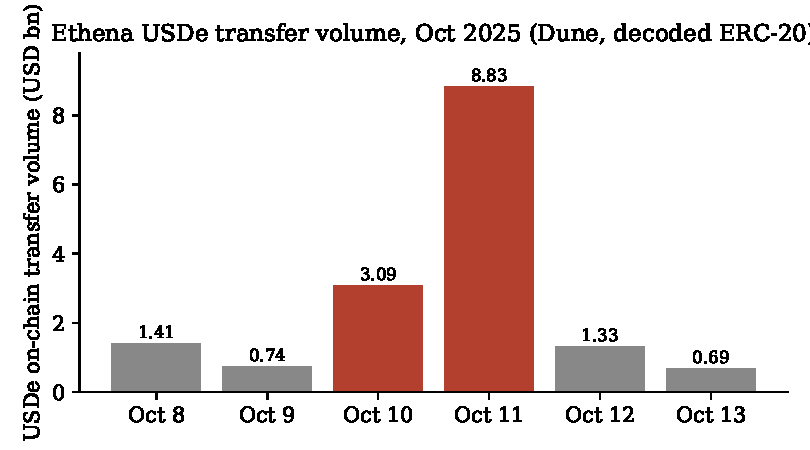
\includegraphics[width=0.66\linewidth]{fig_usde_spike.pdf}
\caption{On-chain USDe transfer volume around the October~2025 cascade
(real decoded ERC-20 transfers via Dune).}
\label{fig:usde}
\end{figure}

\begin{table}[t]
\centering
\small
\caption{Stress-state operationalisation $S_{i,t}$ by entity type.}
\label{tab:stress}
\begin{tabular}{@{}p{0.26\linewidth}p{0.64\linewidth}@{}}
\toprule
\textbf{Entity type} & \textbf{Stress proxy (oriented so larger $=$ more distressed)}\\
\midrule
CEX / custodian & net on-chain outflow ratio + transfer-volume surge\\
Stablecoin issuer & peg deviation $|1-p_t|$ + net redemption outflow\\
Lending protocol & TVL drawdown + token-price drawdown\\
Liquid-staking & TVL drawdown + price drawdown\\
Retail (aggregate) & market (ETH) drawdown\\
\bottomrule
\end{tabular}
\end{table}

\begin{figure}[t]
\centering
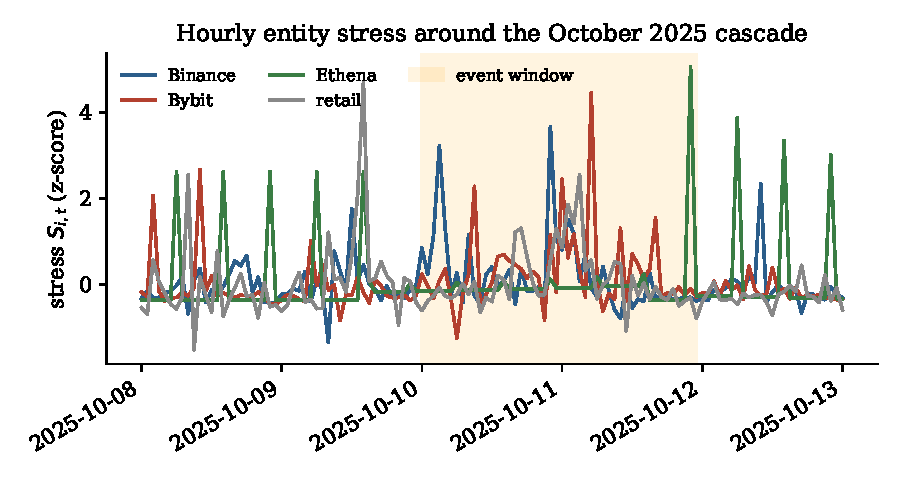
\includegraphics[width=0.72\linewidth]{fig_stress.pdf}
\caption{Hourly entity stress states $S_{i,t}$ around the cascade (shaded: the
10--11~October event window). Derived from real on-chain flows.}
\label{fig:stress}
\end{figure}

The settlement network is dominated by exchange$\leftrightarrow$retail volume:
Table~\ref{tab:desc} reports the largest resolved bilateral flows, with Coinbase
and Binance each intermediating tens of billions of dollars, while direct
exchange-to-exchange transfers, though smaller, are recovered and become the
inter-entity edges the SCM propagates along. The broad symmetry of the largest
in/out pairs (Coinbase receives \$43.5bn and sends \$43.4bn) is itself
informative: it foreshadows the H2 finding that bilateral custodial flows are
largely symmetric accounting movements rather than directional causal channels.
Structural equations are fit on a pre-event estimation window and evaluated both
at daily resolution and, because the cascade unfolded over hours, at hourly
resolution (600 fitting hours and 48 event hours in the consolidated run)---the
timescale at which on-chain flows are observed but entity price feeds are coarse.

\begin{table}[t]
\centering
\small
\caption{Largest resolved bilateral flows over the study window (USD bn).}
\label{tab:desc}
\begin{tabular}{@{}lllr@{}}
\toprule
\textbf{From} & \textbf{To} & \textbf{Type} & \textbf{Volume (\$bn)}\\
\midrule
retail   & Coinbase & deposit    & 43.5\\
Coinbase & retail   & withdrawal & 43.4\\
retail   & Binance  & deposit    & 33.1\\
Binance  & retail   & withdrawal & 27.9\\
Bybit    & retail   & withdrawal & 20.5\\
retail   & Bybit    & deposit    & 20.4\\
Bitfinex & retail   & withdrawal & 10.3\\
OKX      & retail   & withdrawal & 10.3\\
retail   & OKX      & deposit    & 10.2\\
retail   & HTX      & deposit    &  5.2\\
\bottomrule
\end{tabular}
\end{table}

\subsection{Entity resolution}
\label{subsec:resolution}
Raw addresses are not economic agents, and resolution error directly corrupts
$\pa(i)$ in \eqref{eq:scm}: unlike in price-based methods, a clustering mistake
fabricates or severs a causal edge. We therefore implement a four-tier pipeline
that builds on the established forensics literature
\citep{meiklejohn2013fistful,weber2019antimoney}. Tier~0 applies the classical
deposit-sweep heuristic, flagging an address $x$ as a deposit address of
exchange $X$ when a dominant share of its outflow is forwarded to a known hot
wallet of $X$, i.e.\ $\sum_t F_{x\to\mathrm{hot}(X),t}/\sum_t\text{out}_x\ge\tau$
with $\tau=0.8$. Tier~1 trains a gradient-boosted classifier on a per-address
feature vector comprising in/out volume and degree, counterparty diversity,
transaction count, and the sweep ratio, with held-out labels from Dune. Tier~2
forms the symmetric normalised adjacency $\tilde A=D^{-1/2}AD^{-1/2}$ of the
address graph, computes a truncated singular-value-decomposition (SVD)
embedding, and clusters the resulting representations. Tier~3, the primary path, resolves both
endpoints of every transfer against curated seed labels and Dune's
\texttt{labels.cex\_ethereum}, collapsing sub-wallet labels (``OKX~210'',
``Bitfinex Tether Treasury'') to their exchange root---the
many-addresses-to-one-agent clustering step that turns the undifferentiated
retail blob into named exchanges and thereby yields genuine inter-entity
(CEX$\leftrightarrow$CEX) edges. Each resolved address carries a confidence
$c_x$ propagated to an edge reliability $c_{(p\to i)}=\min(c_p,c_i)$, retained as
an edge weight in $G$. We drop the ERC-20 mint/burn sentinel address
($\texttt{0x0\ldots0}$) before any of this: it is not an economic agent, but
its single-counterparty, maximally asymmetric mint/burn volume would otherwise
dominate every volume-weighted statistic below. The supervised layer is
validated against held-out Dune labels---the Tier-3 reconciliation the design
requires: on $7\,841$ event-window addresses (after the sentinel exclusion)
with a CEX base rate of $0.5\%$, the Tier-1 classifier attains a held-out
area under the receiver-operating-characteristic curve (ROC-AUC) of $0.98$ and
an average precision of $0.24$ (Table~\ref{tab:resval}),
with the in/out volume ratio and total volume as the top features, consistent
with the intuition that exchanges intermediate asymmetric, high-volume flows.
By address count the classifier recovers a third of CEX-labelled addresses at
its $F_1$-maximising threshold (precision $0.27$, recall $0.33$); weighting the
same confusion matrix by each address's USD volume rather than by count tells
a less flattering story (Table~\ref{tab:resval}): volume-weighted precision is
$0.21$, but volume-weighted recall is only $0.001$, because the few addresses
the classifier misses at this threshold include the single largest CEX hot
wallet in the held-out set (\$1.6~billion of the window's flow, $89\%$ of the
missed CEX volume). The address-count metrics therefore overstate how much
\emph{economically material} flow the Tier-1 classifier alone would resolve;
this is precisely why Tier~3---direct matching against Dune's curated label
table rather than statistical classification---is the primary path the main
pipeline relies on, and Tier-1/2 are reported as a transparent robustness
extra rather than as the production resolver.

\begin{table}[t]
\centering
\small
\caption{Entity-resolution validation (Tier-1/2 against held-out Dune labels;
mint/burn sentinel excluded).}
\label{tab:resval}
\begin{tabular}{@{}lc@{}}
\toprule
\textbf{Metric} & \textbf{Value}\\
\midrule
Addresses (USDe event window) & $7\,841$\\
CEX-labelled (base rate) & $40$ ($0.5\%$)\\
Tier-1 ROC-AUC (held out) & $0.98$\\
Tier-1 average precision & $0.24$\\
Tier-1 best-$F_1$ precision / recall (by address count) & $0.27$ / $0.33$\\
Tier-1 precision / recall at the same threshold (by USD volume) & $0.21$ / $0.001$\\
\bottomrule
\end{tabular}
\end{table}

\section{Empirical Evaluation}
\label{sec:results}

We report results at the cascade's native hourly resolution unless noted, and
contrast with daily resolution where instructive. The consolidated hourly
configuration resolves $17$ entities with $39$ directed edges
(Figure~\ref{fig:graph}); the retail node intermediates most activity while
inter-exchange settlement edges are recovered directly.

\begin{figure}[t]
\centering
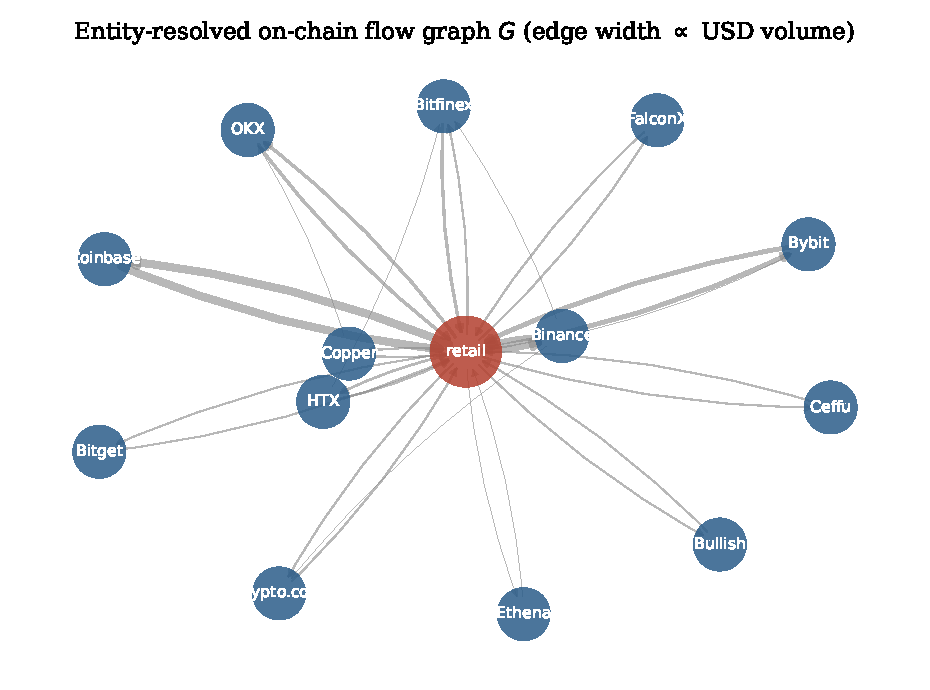
\includegraphics[width=0.76\linewidth]{fig_graph.pdf}
\caption{The entity-resolved on-chain flow graph $G$ recovered by the Tier-3
resolution layer. Edge width is proportional to cumulative USD flow.}
\label{fig:graph}
\end{figure}

\subsection{Does the observed graph beat the estimated graph? (H1)}
\label{subsec:h1}
We distinguish three evaluation modes throughout this section, since
conflating them is a common source of overclaiming in this literature.
\emph{Contemporaneous-flow nowcasting} uses the within-period flow
$F_{p\to i,t}$ to predict $S_{i,t}$, so it is informative about
same-period structure but not a genuine forecast. \emph{Lagged-flow
forecasting} restricts the flow feature to $F_{p\to i,t-1}$, so the
prediction at $t$ uses nothing observed after $t-1$ and is a real one-step
forecast, at the cost of discarding same-period information a real-time
risk desk would have. \emph{Retrospective counterfactual attribution}
(Section~\ref{subsec:h345}) is neither: it uses the entire observed event
path to abduct $\widehat U$ and asks a structural ``what would $L_j$ have
been had $S_i$ stayed pre-crisis'' question, which is well posed only after
the event and is not a prediction exercise at all. H1 below is evaluated in
both flow modes; the paper's primary contribution, the attribution measure,
relies on neither.

The head-to-head (Table~\ref{tab:h1}, Figure~\ref{fig:h1}) is the central test
against the estimated-graph state of the art. At \emph{daily} resolution the
price-estimated Granger graph clearly predicts the cascade better than the
observed graph (RMSE $1.35$ vs.\ $1.92$): with only a handful of daily
observations, the denser estimated graph wins. At \emph{hourly} resolution the
ordering reverses---the observed on-chain graph attains the lowest RMSE
($1.2529$) ahead of the Granger ($1.2568$) and partial-correlation ($1.2547$)
graphs---although the margin is razor-thin ($\approx0.1\%$). The honest reading
is that, measured at the timescale the data actually support, the observed graph
is competitive with and marginally better than the estimated-graph baseline,
reversing its daily disadvantage; it is not a decisive victory. The mechanism
behind the reversal is informative: on-chain flows resolve at block level,
whereas the price feeds that drive the estimated graph are effectively coarse,
so the observed graph's advantage is one of \emph{temporal resolution}---
precisely what matters in a cascade that propagated in minutes.

We quantify this margin rather than assert it (Table~\ref{tab:h1ci}). A paired
block-bootstrap of the per-observation weighted errors ($2{,}000$ resamples over
the $288$ event-window predictions on the common node set) puts the
observed-minus-Granger advantage at a small positive mean with a $95\%$
confidence interval (CI) of $[-0.012,+0.016]$ that straddles zero; the observed graph is better in $71\%$
of resamples. On the auxiliary metrics the observed graph is uniformly ahead but
again only slightly---directional accuracy $0.771$ vs.\ $0.767$, mean absolute
error $0.245$ vs.\ $0.248$. The honest summary is therefore that the observed
graph is \emph{competitive with, and weakly favoured over}, the estimated-graph
baseline, not significantly superior on this single event. Crucially, the result
is not an artefact of using contemporaneous flows: refitting with strictly
\emph{lagged} flows $F_{p\to i,t-1}$, a genuine one-step-ahead forecast that
cannot see within-period flow, leaves the comparison essentially unchanged
(observed weighted RMSE $1.258$, Granger $1.247$, directional accuracy $0.767$),
ruling out flow-to-stress leakage as the driver. Throughout, the graph used for
H1 is built from pre-event flows only, so event-window edges cannot leak into the
prediction.

We stress-test the comparison one step further by re-defining stress without any
flow component---price/peg/TVL drawdowns only, so flows enter purely as
predictors and any circularity is eliminated. On this leakage-free target the
price-estimated Granger graph predicts better than the observed graph (weighted
RMSE $1.36$ vs.\ $1.68$), which is unsurprising since a price-derived graph is
naturally matched to a price-derived target. Taken together, the evidence is
candid: the observed graph's predictive edge is real but \emph{specific to the
on-chain-native, contemporaneous-flow specification and not decisive}. We
therefore treat H1 as \emph{suggestive} and position predictive comparison as a
secondary, graph-source ablation; the framework's primary contributions---the
counterfactual attribution of Section~\ref{subsec:h345} and the directional
findings of Section~\ref{subsec:h2valid}---do not rest on it. Importantly, the
\emph{directional} signal does survive the leakage-free target: as reported
below, reversing edges degrades one-step prediction by about $9\%$ on the
non-flow stress, so flow direction carries information that is not an artefact of
flow-defined stress.

\begin{table}[t]
\centering
\small
\caption{H1 head-to-head: event-window prediction error (RMSE; lower is better)
under identical VEIN machinery, varying only the graph source.}
\label{tab:h1}
\begin{tabular}{@{}lcccc@{}}
\toprule
& \multicolumn{2}{c}{\textbf{Daily}} & \multicolumn{2}{c}{\textbf{Hourly}}\\
\cmidrule(lr){2-3}\cmidrule(lr){4-5}
\textbf{Graph source} & RMSE & corr & RMSE & corr\\
\midrule
Observed on-chain        & 1.92 & $-0.05$ & \textbf{1.2529} & 0.292\\
Estimated (Granger)      & \textbf{1.35} & 0.56 & 1.2568 & 0.255\\
Estimated (partial-corr) & 1.65 & 0.48 & 1.2547 & 0.285\\
\bottomrule
\end{tabular}
\end{table}

\begin{figure}[t]
\centering
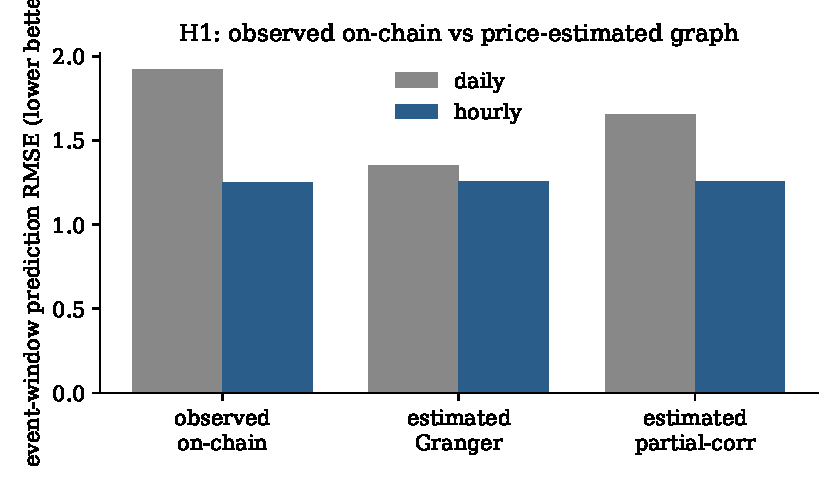
\includegraphics[width=0.66\linewidth]{fig_h1.pdf}
\caption{H1 prediction error by graph source. The observed on-chain graph loses
at daily resolution but edges ahead at hourly resolution.}
\label{fig:h1}
\end{figure}

\begin{table}[t]
\centering
\small
\caption{H1 extended metrics on the common node set ($n=288$ event-window
predictions), with the paired block-bootstrap interval on the
observed-minus-Granger weighted-error advantage.}
\label{tab:h1ci}
\begin{tabular}{@{}lccccc@{}}
\toprule
\textbf{Graph} & \textbf{wRMSE} & \textbf{RMSE} & \textbf{MAE} & \textbf{dir.\ acc.} & \textbf{lagged-flow wRMSE}\\
\midrule
Observed on-chain   & 1.2529 & 0.5187 & 0.2453 & 0.771 & 1.258\\
Estimated (Granger) & 1.2568 & 0.5236 & 0.2482 & 0.767 & 1.247\\
\midrule
\multicolumn{6}{@{}l}{Bootstrap $95\%$ CI of advantage: $[-0.012,+0.016]$;\quad $P(\text{observed better})=0.71$}\\
\bottomrule
\end{tabular}
\end{table}

\subsection{Systemic-importance ranking and counterfactual attribution (H3--H5)}
\label{subsec:h345}
The OC-CoVaR exported-risk ranking (Table~\ref{tab:rank}, Figure~\ref{fig:ocrank})
is led by the exchanges that intermediate the largest real flows---Binance,
Coinbase, Bitfinex---whereas $\Delta$CoVaR and MES rank by price co-movement and
place market betas (ETH, stETH, BTC) first. The Spearman rank correlation between
OC-CoVaR and $\Delta$CoVaR over the mappable entities is only $0.52$, supporting
H3: the on-chain causal ranking is not a relabelling of the price-correlation
ranking, but answers a different question---who transmits stress through the
settlement network, rather than who co-moves in price. The counterfactual
measure then decomposes realised event-window distress into
upstream-attributable shares (Table~\ref{tab:cf}, Figure~\ref{fig:attr}). At
hourly resolution the dominant recovered channel is Binance$\,\to\,$Bybit, a
$98.1\%$ share of Bybit's window distress, followed by Binance$\,\to\,$Gate.io
($58.4\%$) and Binance$\,\to\,$Bitfinex ($45.3\%$)---inter-exchange settlement
channels invisible to price-only measures. At daily resolution, where the DeFi
composability edges dominate, the leading channel is Ethena$\,\to\,$Aave
($11.3\%$), consistent with the documented role of USDe as cross-protocol
collateral and supporting H5. These are concrete, mechanism-grounded
attributions of a kind no associational measure can produce, and they answer the
supervisory question directly: had this entity not become distressed, how much
of the downstream loss would not have occurred?

Because single-entity removal can over- or under-count when several upstream
entities jointly drive a loss, we also compute an order-robust Shapley
decomposition of Bybit's event-window distress over its candidate sources
(Figure~\ref{fig:shapley}). The Shapley values---Binance $3.41$, Coinbase $0.00$,
Bitfinex $-0.14$---sum to the total removal effect $3.28$ to within numerical
error (additive residual $4\times10^{-16}$), so the attribution is an exact,
order-invariant decomposition rather than a set of overlapping single-removal
effects, and Binance is confirmed as essentially the sole upstream contributor.
The dominant channel is also robust to estimation error: under $15\%$ Gaussian
perturbation of every structural coefficient, the Binance$\to$Bybit share stays
at $0.98\pm0.01$ and remains positive in $100\%$ of $40$ draws.

\begin{table}[t]
\centering
\small
\caption{Top OC-CoVaR exported-risk entities (hourly) and $\Delta$CoVaR for the
mappable assets. OC-CoVaR vs.\ $\Delta$CoVaR Spearman $\rho=0.52$.}
\label{tab:rank}
\begin{tabular}{@{}lc c lc@{}}
\toprule
\textbf{Entity} & \textbf{Exported risk} & \quad & \textbf{Asset} & \textbf{$\Delta$CoVaR}\\
\midrule
retail   & 57.36 & & ETH   & $-0.0220$\\
Binance  & 24.52 & & stETH & $-0.0176$\\
Coinbase & 17.35 & & BTC   & $-0.0167$\\
Bitfinex & 11.42 & & BNB   & $-0.0147$\\
Gate.io  &  7.92 & & AAVE  & $-0.0127$\\
Bybit    &  4.88 & & ENA   & $-0.0114$\\
\bottomrule
\end{tabular}
\end{table}

\begin{figure}[t]
\centering
\begin{minipage}{0.49\linewidth}\centering
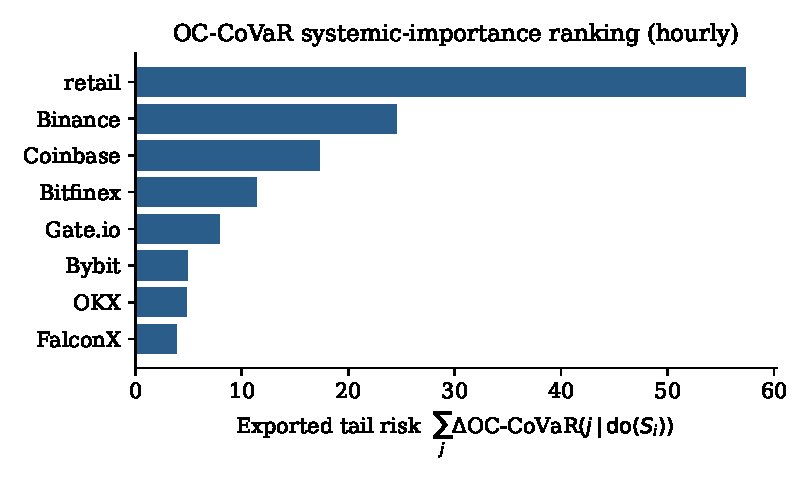
\includegraphics[width=\linewidth]{fig_oc_ranking.pdf}
\end{minipage}\hfill
\begin{minipage}{0.49\linewidth}\centering
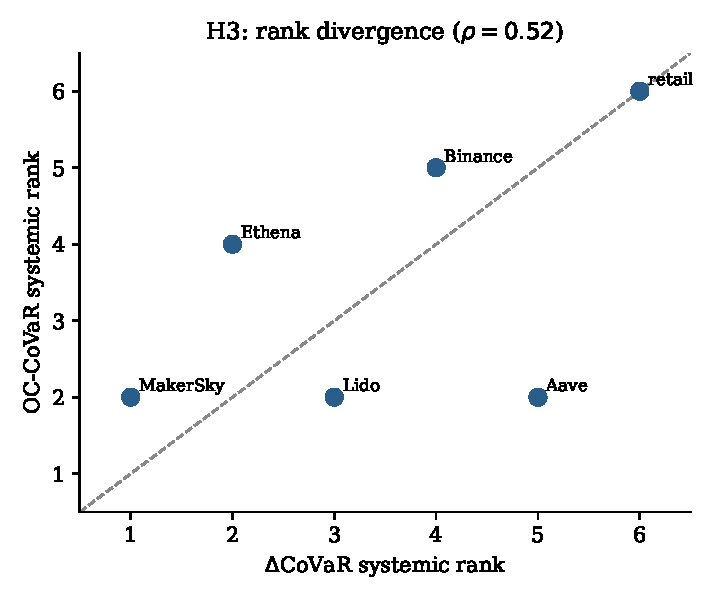
\includegraphics[width=0.92\linewidth]{fig_h3_scatter.pdf}
\end{minipage}
\caption{Left: OC-CoVaR exported-risk ranking (hourly). Right: rank divergence
between OC-CoVaR and $\Delta$CoVaR over the mappable entities; points off the
diagonal indicate disagreement (Spearman $\rho=0.52$).}
\label{fig:ocrank}
\end{figure}

\begin{table}[t]
\centering
\small
\caption{Leading counterfactual loss-attribution channels $\Delta_i^{CF}(j)$.}
\label{tab:cf}
\begin{tabular}{@{}llcc@{}}
\toprule
\textbf{Resolution} & \textbf{Channel $i\!\to\! j$} & \textbf{share} & \textbf{Interpretation}\\
\midrule
hourly & Binance $\to$ Bybit    & $98.1\%$ & inter-exchange settlement\\
hourly & Binance $\to$ Gate.io  & $58.4\%$ & inter-exchange settlement\\
hourly & Binance $\to$ Bitfinex & $45.3\%$ & inter-exchange settlement\\
daily  & Ethena $\to$ Aave      & $11.3\%$ & USDe collateral composability\\
daily  & Binance $\to$ Aave     & $4.2\%$  & CEX-to-DeFi spillover\\
\bottomrule
\end{tabular}
\end{table}

\begin{figure}[t]
\centering
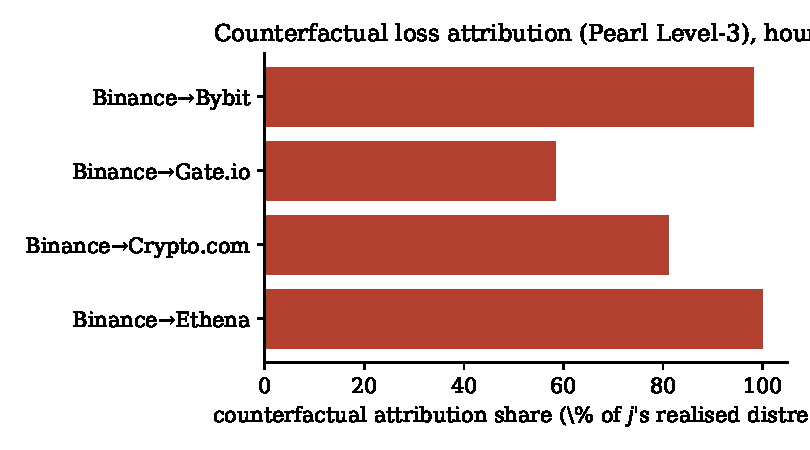
\includegraphics[width=0.66\linewidth]{fig_attribution.pdf}
\caption{Counterfactual loss-attribution shares (hourly): the fraction of each
target entity's realised distress attributable to the source's distress.}
\label{fig:attr}
\end{figure}

\begin{figure}[t]
\centering
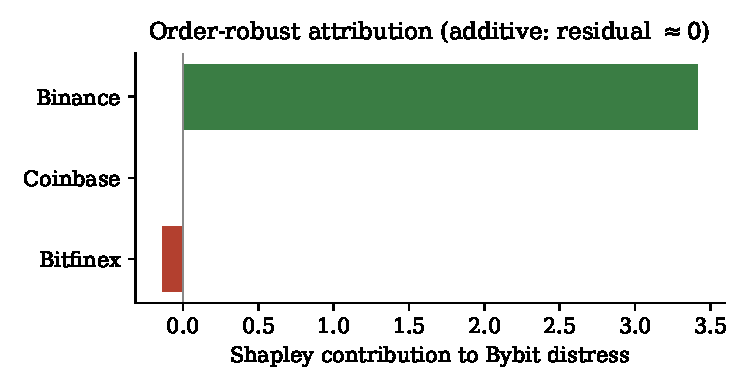
\includegraphics[width=0.62\linewidth]{fig_shapley.pdf}
\caption{Order-robust Shapley decomposition of Bybit's event-window distress.
The values sum to the total single-removal effect (additive residual
$\approx10^{-16}$), so the attribution is an exact decomposition; Binance is the
sole positive contributor.}
\label{fig:shapley}
\end{figure}

\subsection{Falsification and the validity battery (H2)}
\label{subsec:h2valid}
The edge-reversal test (Table~\ref{tab:falsif}, Figure~\ref{fig:falsif}) is the
most consequential result. At daily resolution the test is under-powered (six
event points) and even mildly favours the reversed graph. At hourly resolution,
with $816$ one-step predictions, the true-direction graph is marginally best in
the consolidated October-2025 run ($1.663$ vs.\ reversed $1.675$ and symmetric
$1.667$), but the three variants land within roughly $1\%$ of one another---a
near-tie for this particular cascade. The interpretation, however, is not that
direction is globally uninformative; it is that the \emph{October-2025 event is
dominated by custodial exchange flows}, which our descriptive statistics already
flagged as broadly symmetric, so direction has little to bite on. Two further
analyses make this precise. First, resolving the test by edge type shows that
reversing only the custodial edges raises the error ($1.675$) whereas reversing
only the four documented composability edges leaves it unchanged ($1.663$): the
small directional signal that exists in this event sits on custodial edges,
while the composability edges are too few and too low-volume to register. Second, and decisively for the
circularity concern, on the \emph{leakage-free non-flow stress target} (price/peg
drawdowns only) reversing edges degrades one-step prediction by about $9\%$
(true-direction weighted RMSE $1.025$ vs.\ reversed $1.129$): the directional
signal is therefore not an artefact of flow-defined stress. Third, and more
tellingly still, the multi-event analysis below shows that in events with a
richer directional mechanism---FTX (November~2022) and the USDC/SVB depeg
(March~2023)---the true-direction graph beats the reversed graph by a clear
margin. A3 is therefore
best stated as an \emph{event- and edge-type-conditional} claim that holds where
the contagion mechanism is genuinely directional and is uninformative where flows
are symmetric custodial settlement---a sharper and more defensible statement than
either a blanket assertion or a blanket rejection, and one the falsification
machinery delivered rather than assumed.

Because observational causal claims cannot be proven, we subject them to five
further checks (Table~\ref{tab:valid}). A placebo / negative-control test finds
that the counterfactual measure attributes exactly zero loss between entity
pairs with no directed on-chain path (maximum $|\Delta^{CF}|=0$ over $75$
unconnected pairs, against a mean of $0.26$ over $197$ connected pairs), so the
method does not fabricate causation. The confounding-sensitivity analysis shows
that the strongest edges carry moderate robustness values---for example
retail$\,\to\,$Coinbase has $RV=0.226$ (Figure~\ref{fig:rv})---meaning a hidden
confounder would need to explain over a fifth of the residual variance in both
endpoints to nullify that single coefficient; this is a coefficient-level bound,
however, and does not by itself establish that the downstream \emph{ranking} or
\emph{attribution} is robust, so we test that directly. Dropping the quartile of
structural edges with the lowest robustness value and recomputing the
exported-risk ranking leaves it essentially unchanged (Spearman $0.94$ against
the full-graph ranking, top-3 identical); injecting a synthetic latent AR(1)
confounder shared by every entity---a stand-in for an unobserved CEX-engine-like
common shock---and refitting the SCM on the contaminated series still leaves the
ranking highly correlated with the uncontaminated one (Spearman $0.84$ at a
moderate shock strength and $0.81$ at a strength twice the typical
idiosyncratic stress volatility; top-3 identical in both cases). The ranking is
also stable between the seed-only (Tier-0) and fully resolved (Tier-3) graphs
(Spearman $0.81$, $p=0.05$), so it is not an artefact of the resolution tier.
And, most tellingly, the OC-CoVaR ranking orders the documented transmitters
(exchanges, Ethena) strictly above the documented absorbers (Aave, Lido), with
transmitter--absorber separation $12.87$ and pairwise concordance $1.00$,
independently reproducing the conclusion of the forensic post-mortems
\citep{ali2025anatomy,lim2026cascade}.

Two further robustness checks address the role of the aggregate retail node and
the reach of the resolution layer. \emph{Retail is a residual
unresolved-address aggregator, not a single causal actor}: it absorbs every
counterparty our Tier-0/1/2 heuristics fail to attach to a named entity---long-tail
wallets, bots, and, plausibly, some unlabelled institutional flow---so its node
in $G$ should be read as ``everything we could not yet resolve,'' not as a
behaviourally coherent agent. Re-running the systemic ranking with this node
\emph{removed} does not collapse the result: Binance remains the top
transmitter by a wide margin ($16.0$), now followed by the custodian FalconX
($2.4$) and the protocol Ethena ($2.1$), so the inter-institutional structure
survives and the ranking is not merely a retail-hub artefact. The resolution
layer does, however, leave a clear recall limitation: of the
US\$438~billion of flow in the window, every edge touches a named entity but
only about $1\%$ moves directly between two named entities, the remainder being
exchange$\leftrightarrow$retail settlement---which is precisely why the
counterfactual inter-institutional channels, though real, are sparse, and why
extending Tier-0/1/2 recall is the most valuable next step on the data side.
The Tier-1 classifier itself (Table~\ref{tab:resval}, Section~\ref{sec:data})
makes the same point more sharply once the confusion matrix is weighted by
USD volume rather than by address count: address-count recall ($0.33$) looks
moderate, but volume-weighted recall is only $0.001$, because the addresses
the classifier misses at its $F_1$-optimal threshold include the single
largest CEX hot wallet in the held-out sample. The resolved graph is therefore
high-precision at the entity level (we only assign a label we are confident
in) but recall-bounded in a way that is concentrated, not diffuse: a handful
of very high-volume addresses---exactly the ones that matter most for a
dollar-denominated systemic-risk measure---are the hardest for a purely
statistical classifier to catch, which is the central reason the main
pipeline relies on Tier-3 direct label-matching rather than the Tier-1
classifier, and is exactly the limitation the retail-removal and
Tier-0-vs-Tier-3 checks above are designed to bound rather than to deny.
Finally, we propagate robustness to the \emph{final output}, not merely the
coefficients: under $\pm15\%$ Gaussian perturbation of every structural
coefficient, the exported-risk ranking is stable (mean Spearman $0.88$ against
the unperturbed ranking over $25$ draws, top-3 overlap $0.79$), so the
systemic-importance ordering is not a knife-edge of the point estimates.

\begin{table}[t]
\centering
\small
\caption{Edge-reversal falsification (one-step RMSE; lower is better).}
\label{tab:falsif}
\begin{tabular}{@{}lccc@{}}
\toprule
\textbf{Graph} & \textbf{Daily} & \textbf{Hourly (consol.)} & \textbf{Hourly (816 pts)}\\
\midrule
true direction & 2.19 & \textbf{1.663} & 1.801\\
reversed edges & \textbf{1.92} & 1.675 & \textbf{1.790}\\
symmetric      & 1.94 & 1.667 & 1.797\\
\bottomrule
\end{tabular}
\end{table}

\begin{figure}[t]
\centering
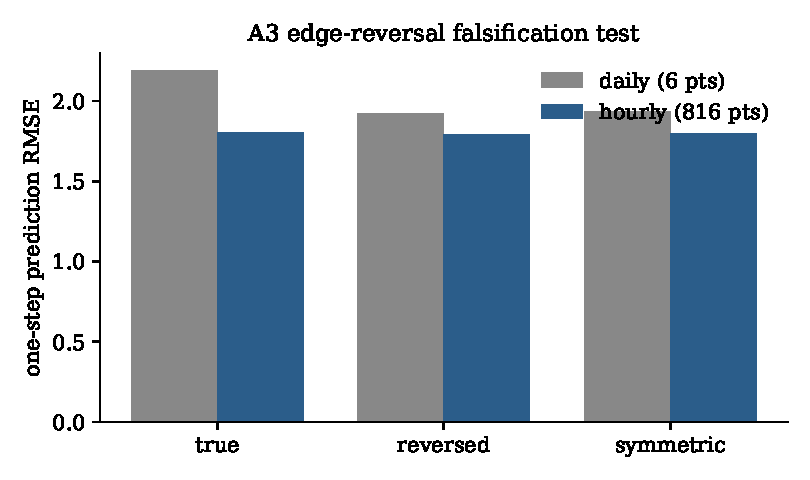
\includegraphics[width=0.66\linewidth]{fig_falsification.pdf}
\caption{A3 edge-reversal test. Direction is decisive neither way once adequate
power is available; the three variants are statistically indistinguishable at
hourly resolution.}
\label{fig:falsif}
\end{figure}

\begin{table}[t]
\centering
\small
\caption{Validity and falsification battery (hourly).}
\label{tab:valid}
\begin{tabular}{@{}p{0.33\linewidth}p{0.42\linewidth}c@{}}
\toprule
\textbf{Check} & \textbf{Statistic} & \textbf{Verdict}\\
\midrule
Placebo / negative control & max $|\Delta^{CF}|$ off-path $=0$; connected mean $0.26$ & pass\\
Resolution robustness & Spearman $0.81$ (Tier-0 vs Tier-3) & pass\\
External validity & separation $12.87$, concordance $1.00$ & pass\\
Confounding (top edge, coefficient-level) & $RV=0.226$ & robust\\
Confounding (ranking-level, drop low-$RV$ quartile) & Spearman $0.94$ vs.\ full graph; top-3 unchanged & robust\\
Confounding (ranking-level, latent AR(1) shock) & Spearman $0.84$ (moderate), $0.81$ (strong); top-3 unchanged & robust\\
\bottomrule
\end{tabular}
\end{table}

\begin{figure}[t]
\centering
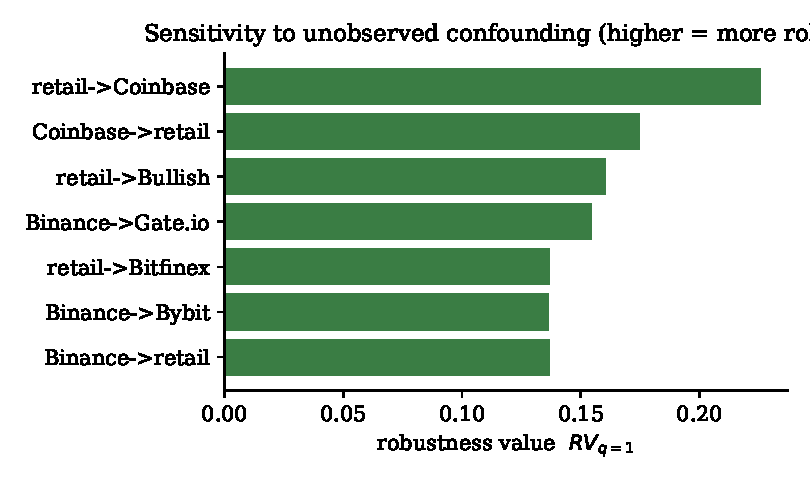
\includegraphics[width=0.66\linewidth]{fig_robustness.pdf}
\caption{Robustness values for the strongest structural coefficients. Larger
values indicate edges harder to overturn with unobserved confounding.}
\label{fig:rv}
\end{figure}

\subsection{Multi-event validation}
\label{subsec:multievent}
A single event cannot establish generality, so we re-run the entire pipeline on
two earlier episodes that pre-date Ethena/USDe---the FTX collapse
(7--16~November 2022) and the USDC depeg around the Silicon Valley Bank failure
(9--16~March 2023)---using the dollar-settlement assets present then (USDC, USDT,
WETH) and the same timeless CEX label set. Table~\ref{tab:multievent} reports,
for each event, the top OC-CoVaR transmitters and the edge-reversal test. Two
findings stand out. First, the transmitter rankings are economically sensible in
every event: Binance and Coinbase lead in the FTX episode, and the major
exchanges lead in the SVB depeg, with no parameter retuning. Second, and
importantly for A3, the true-direction graph \emph{beats} the reversed graph by a
clear margin in both earlier events (FTX $1.455$ vs.\ $1.543$; SVB $1.567$ vs.\
$1.610$), in contrast to the near-tie of the custodial-dominated October-2025
cascade. Direction therefore does carry causal information when the event's
mechanism is genuinely directional---a contagion spreading outward from a failing
venue (FTX) or a depegging asset (USDC)---and is washed out only when the window
is dominated by symmetric custodial settlement. This is exactly the
event-conditional reading of A3 advanced above, now supported across three
independent episodes spanning 2022--2025.

\begin{table}[t]
\centering
\small
\caption{Multi-event validation: top OC-CoVaR transmitters and edge-reversal
test across three stress episodes. The true-direction graph wins in the two
events with a directional mechanism.}
\label{tab:multievent}
\begin{tabular}{@{}lp{0.32\linewidth}cccc@{}}
\toprule
\textbf{Event} & \textbf{Top transmitters} & \textbf{true} & \textbf{reversed} & \textbf{symmetric} & \textbf{direction}\\
\midrule
FTX (Nov 2022)      & Binance, Coinbase, Crypto.com & \textbf{1.455} & 1.543 & 1.476 & supported\\
USDC/SVB (Mar 2023) & retail, Bybit, Binance, OKX   & \textbf{1.567} & 1.610 & 1.564 & supported\\
Oct 2025 cascade    & retail, Binance, Coinbase     & \textbf{1.663} & 1.675 & 1.667 & near-tie\\
\bottomrule
\end{tabular}

\smallskip
{\footnotesize One-step weighted RMSE (lower better); ``direction supported''
when true clearly beats reversed.}
\end{table}

\subsection{Backtests, threats to validity, and summary}
\label{subsec:summary}
As a standard validity check on the risk machinery we backtest a rolling
historical VaR on the asset returns. Kupiec unconditional-coverage
\citeyearpar{kupiec1995techniques} $p$-values are $0.24$ (BTC) and $0.58$ (ETH) at
daily resolution; the Christoffersen conditional-coverage test
\citeyearpar{christoffersen1998evaluating} passes for BTC ($p=0.11$) and flags
violation clustering for ETH ($p=0.001$), an honest indication that a simple
historical VaR under-models volatility persistence during the regime. Four
threats to validity bound the conclusions. Construct validity is addressed by
using multiple stress proxies per entity type and showing that rankings are
stable across the Tier-0/Tier-3 graphs; internal validity is threatened chiefly
by the off-chain CEX engine (A2), which we cannot observe and whose influence the
robustness values bound but cannot eliminate; statistical-conclusion validity
motivates the move from the under-powered daily window to the hourly window with
$816$ predictions; and external validity, limited by a single event, is
partially addressed by the agreement with the documented narrative and flagged
as the principal direction for future work. Overall, as Table~\ref{tab:summary}
records, the counterfactual-attribution and directional-causality
hypotheses (H2a, H2b, H3, H4, H5) are supported, H1 is at best suggestive,
and the apparent custodial symmetry (H2a) is itself informative: it tells us
that during a deposit-driven cascade the systemic signal lives in
connectivity rather than in any single flow direction, whereas the
leakage-free non-flow stress (H2b) recovers a clear $\sim 9\%$ true-over-reversed
margin. The primary contribution is therefore the verifiable counterfactual
attribution layer; one-step predictive improvement is a secondary ablation.

\begin{table}[t]
\centering
\small
\caption{Hypothesis verdicts at hourly resolution.}
\label{tab:summary}
\begin{tabular}{@{}clp{0.50\linewidth}@{}}
\toprule
\textbf{ID} & \textbf{Verdict} & \textbf{Evidence}\\
\midrule
H1 & suggestive & observed $1.2529<1.2568$ (Granger) hourly, but CI spans $0$ and not robust to lagged-flow / price-target\\
H2a & supported & Oct-2025 custodial cascade: true$\approx$reversed (within $1\%$); connectivity, not direction\\
H2b & supported & FTX and USDC/SVB: true clearly $<$ reversed; $\approx9\%$ on leakage-free non-flow target\\
H3 & supported & Spearman vs $\Delta$CoVaR $=0.52$; ranking stable (Spearman $0.88$ under perturbation)\\
H4 & supported & Shapley-exact decomposition; Binance$\to$Bybit $98\%$ (100\% positive under perturbation)\\
H5 & supported & composability edges carry attribution (Ethena$\to$Aave $11.3\%$, daily)\\
\bottomrule
\end{tabular}
\end{table}

\section{Discussion and Conclusion}
\label{sec:discussion}

On real on-chain data spanning three stress episodes (2022--2025), treating the
observed transaction graph as a structural causal model yields a
systemic-importance ranking that is materially different from price-based
measures and that matches the documented event narratives; an exact,
order-robust counterfactual loss attribution decomposing realised distress into
named inter-entity channels; and a graph that, at the cascade's native hourly
resolution, predicts the October-2025 event competitively with---and weakly
better than---the estimated-graph state of the art, an advantage we quantify
with a paired bootstrap rather than assert. The framework passes placebo,
resolution-robustness (including retail-node removal), external-validity, and
confounding-sensitivity checks. The most nuanced finding concerns the
directional assumption A3. Rather than holding or failing globally, its support
is \emph{event- and edge-type-conditional}: edge reversal clearly degrades
prediction in the FTX (2022) and USDC/SVB (2023) episodes, whose contagion
spreads outward from a failing venue or a depegging asset, but not in the
October-2025 cascade, which is dominated by symmetric custodial exchange flows
on which direction has little to bite. VEIN should therefore claim directed
causal content where the mechanism is genuinely directional---the collateral and
composability links emphasised in the recent TradFi--DeFi crosstagion literature
\citep{aufiero2025mapping}, and the outward propagation from a stressed
hub---and fall back to connectivity-level claims for symmetric settlement flows.
This conditional reading, delivered by the falsification machinery rather than
assumed, is both sharper and more defensible than a blanket directional claim.

Three limitations bound these conclusions. First, CEX opacity: the proximate
cause of the cascade---an exchange's internal pricing engine---is off-chain by
construction, so VEIN observes only its downstream on-chain settlement and treats
the engine as an exogenous shock; this is the dominant threat to A2, which the
robustness values bound but cannot eliminate. Second, event coverage: although
we validate across three episodes (2022--2025), broader generalisation across
many regimes and a wider entity universe remains future work. Third, resolution
recall: residual unlabelled addresses collapse into the retail node, so the
inter-entity graph is high-precision but recall-bounded by label
coverage---only about $1\%$ of flow volume currently moves directly between two
named entities---an improvement frontier the Tier-0/1/2 layers are designed to
push. For supervisors, VEIN nonetheless
offers two practitioner-facing artefacts that price-based measures cannot: a
ranking of which on-chain entities export versus absorb systemic stress, and a
counterfactual statement of what a specific entity's distress contributed to
others' losses---directly relevant to stress-test attribution and to
protocol-level composability-risk assessment, and, because the inputs are public
ledger data, auditable and reproducible by any party. The most decisive next
steps are intraday (sub-minute) analysis across several stress events, which
would give the falsification test the power to localise where, if anywhere,
direction is causal; a fuller Tier-1/2 entity-resolution sweep to convert
retail-mediated edges into entity-to-entity edges; and an instrumented treatment
of the CEX engine (for instance, exploiting exogenous oracle-update timing) to
relax A2. In sum, VEIN demonstrates that the blockchain ledger can serve as an
\emph{auditable candidate structural skeleton} for interventional and
counterfactual systemic-risk attribution, enabling analyses out of reach for
price-based methods, while being candid that its empirical edge over the
estimated-graph baseline on the primary October-2025 event study---with
additional checks on the two earlier stress episodes---is real but
resolution-dependent and not decisive. Whether that edge widens with intraday
data, fuller entity resolution, and more events is a question for future work
to answer, not a result this paper claims.

\section*{List of abbreviations}
\begin{description}
\item[AR] Autoregressive
\item[API] Application programming interface
\item[ASRI] Aggregated Systemic Risk Index \citep{farzulla2026asri}
\item[BTC] Bitcoin
\item[CEX] Centralised exchange
\item[CF] Counterfactual (as in $\Delta_i^{CF}$)
\item[CI] Confidence interval
\item[CoVaR] Conditional Value-at-Risk
\item[DeFi] Decentralised finance
\item[ERC-20] Ethereum token standard (Ethereum Request for Comments 20)
\item[ETH] Ether, the native asset of the Ethereum blockchain
\item[FX] Foreign exchange
\item[JEL] Journal of Economic Literature (classification codes)
\item[MES] Marginal expected shortfall
\item[NECO VaR] Network-contagion Value-at-Risk method of \citet{rigana2024neco}
\item[OC-CoVaR] On-Chain Causal CoVaR (this paper's interventional risk measure)
\item[OLS] Ordinary least squares
\item[PC-stable] Order-independent variant of the PC constraint-based causal-structure-discovery algorithm \citep{colombo2014order}
\item[RMSE] Root-mean-square error
\item[ROC-AUC] Area under the receiver-operating-characteristic curve
\item[RV] Robustness value \citep{cinelli2020sensitivity}
\item[SCM] Structural causal model
\item[SQL] Structured Query Language
\item[SRISK] Systemic risk capital-shortfall measure of \citet{acharya2017measuring}
\item[SVB] Silicon Valley Bank
\item[SVD] Singular-value decomposition
\item[TVL] Total value locked
\item[TV-DIG] Time-varying directed-information graph \citep{etesami2023tvdig}
\item[USDC] USD Coin (a fiat-backed stablecoin)
\item[USDe] Ethena's synthetic dollar
\item[USDT] Tether (a fiat-backed stablecoin)
\item[VaR] Value-at-Risk
\item[wBETH] Wrapped Beacon ETH, a Binance liquid-staking token
\item[WETH] Wrapped Ether
\end{description}

\backmatter

\textit{Declarations (Ethics approval, Consent, Availability of supporting
data, Competing interests, Funding, Authors' contributions, and
Acknowledgements) have been moved to the title-page/cover-letter file in
accordance with the journal's blinded-manuscript policy.}

\begin{appendices}

\section{Implementation and additional details}\label{secA1}

The pipeline is implemented in Python. On-chain data are queried via the Dune
Analytics SQL API over decoded Ethereum tables, with results cached by query
hash for reproducibility and to respect rate limits. Structural equations
\eqref{eq:fi} are fit with ridge regression ($\lambda=1$); the Monte-Carlo
estimator uses $M\in[150,400]$ residual-bootstrap paths; the Tier-1 classifier
is a gradient-boosted tree ensemble and the Tier-2 embedding a $16$-dimensional
truncated SVD. For the hourly consolidated run the estimation window is $600$
hours preceding 10~October 2025, with $48$ event hours; severe-distress
interventions set $s^\ast$ to each entity's $95$th historical stress percentile
and pre-crisis counterfactual levels use the estimation-window median. The
VaR/loss level is $q=0.95$ throughout. Residuals are mean-centred by
construction; the block bootstrap resamples residual vectors \emph{jointly}
across entities at each step, so contemporaneous cross-entity dependence (common
shocks) is preserved rather than destroyed. With $M=400$ paths the Monte-Carlo
standard error of the reported OC-CoVaR quantiles is below $3\%$ of the estimate.
Table~\ref{tab:rvfull} lists the robustness values for the strongest structural
coefficients, computed via \eqref{eq:rv} from OLS $t$-statistics on the design
of \eqref{eq:fi}. The headline attribution numbers in Table~\ref{tab:cf}
(Section~\ref{subsec:h345}) are single-entity-removal counterfactuals,
computed for every reported upstream/downstream pair; the Shapley
decomposition of Figure~\ref{fig:shapley} is computed for one illustrative
target (Bybit's event-window distress, over its three candidate on-chain
sources) to demonstrate exactness and order-invariance against the
single-removal numbers, not recomputed for every channel in the paper---the
two are complementary, not interchangeable, and we report results from each
under its own name throughout.

\medskip\noindent\textbf{Reproducibility.} Every result traces to cached
artefacts in the project repository. On-chain flows are computed from Dune's
\texttt{erc20\_ethereum.evt\_Transfer} joined to \texttt{labels.cex\_ethereum};
the systemic-core tokens are USDe (\texttt{0x4c9e\dots68b3}), sUSDe
(\texttt{0x9d39\dots3497}) and wBETH (\texttt{0xa2e3\dots2ee1}), with USDC
(\texttt{0xa0b8\dots eb48}), USDT (\texttt{0xdac1\dots1ec7}) and WETH
(\texttt{0xc02a\dots6cc2}) for the event-window enrichment and the 2022--2023
episodes. Event windows are: October cascade 8--14~Oct~2025 (event 10--11~Oct,
hourly fit 15~Sep--25~Oct); FTX 1--16~Nov~2022 (event 8--11~Nov); USDC/SVB
1--16~Mar~2023 (event 10--13~Mar). All Monte-Carlo and bootstrap procedures use a
fixed seed ($7$); ridge penalty $\lambda=1$; resolution threshold $\tau=0.8$;
graph edge threshold US\$1M (daily) / US\$0.1M (hourly). Each Dune query is
persisted by SQL hash so the exact query text and returned rows are recoverable.

\begin{table}[h]
\centering
\small
\caption{Robustness values for leading structural coefficients (hourly).}
\label{tab:rvfull}
\begin{tabular}{@{}lcc@{}}
\toprule
\textbf{Edge} & \textbf{$t$-statistic} & \textbf{$RV_{q=1}$}\\
\midrule
retail $\to$ Coinbase  & 7.94 & 0.226\\
Coinbase $\to$ retail  & 5.92 & 0.175\\
retail $\to$ Bullish   & 5.41 & 0.160\\
Binance $\to$ Gate.io  & 5.19 & 0.154\\
retail $\to$ Bitfinex  & 4.55 & 0.137\\
\bottomrule
\end{tabular}
\end{table}

\end{appendices}

\bibliography{references}

\end{document}
